\chapter{"staff" szintű felhasználói felületek, és azok működése}
\label{chap:fejezet6}

Ahogy a korábbiakban már leírtam, az alkalmazásban a "Staff" felhasználói szint az orvosokat reprezentálja. Nekik lehetőségük van belenézni bármelyik páciens kezeléstörténetébe, és hozzáférnek a páciensek elérhetőségéhez is. Továbbá megadhatják a saját munkaidejüket, és megnézhetik a saját időpontjaikat dátumonként szűrve. Ugyanakkor időpontfoglaláshoz nincs joguk, nem is lenne lehetséges, mivel az orvosok fiókjaihoz nincs "Patient" példány rendelve.

\section{A "Páciensek" oldal}

Ezen az oldalon az orvos rákereshet bármelyik páciensre név szerint az oldalon lévő kereső segítségével, vagy az "Összes páciens" gombra kattintva visszatérhet az alapértelmezett nézetbe, ami az összes adatbázisban lévő pácienst kilistázza az oldalon látható táblázatba. Az oldal a "patients.html" fájlban lett megvalósítva. Mindegyik páciens kattintható, kattintás hatására az adott páciens adatlapjára jut a felhasználó, ami a "patient.html" oldalon lett megvalósítva. Ezen az oldalon vannak a páciensnek az adatai láthatók amelyikre a felhasználó kattintott, továbbá az összes lefoglalt időpontja és azoknak leírása időrend szerint csökkenő sorrendben. Az oldalon alapértelmezetten minden a páciens által lefoglalt időpont megjelenik, viszont a felhasználónak lehetősége van hónap alapján szűrni őket, ezzel könnyebbé téve a kezeléstörténet vizsgálatát. Az oldalon található még egy "Vissza a páciensekhez" gomb, ami visszavezet a "Páciensek" oldalra. A 6.1. ábrán ennek az oldalnak a kinézete látható.

\begin{figure}[H]
	\caption{A "Páciensek" oldal}
	\label{fig:paciensek}
	\centering
	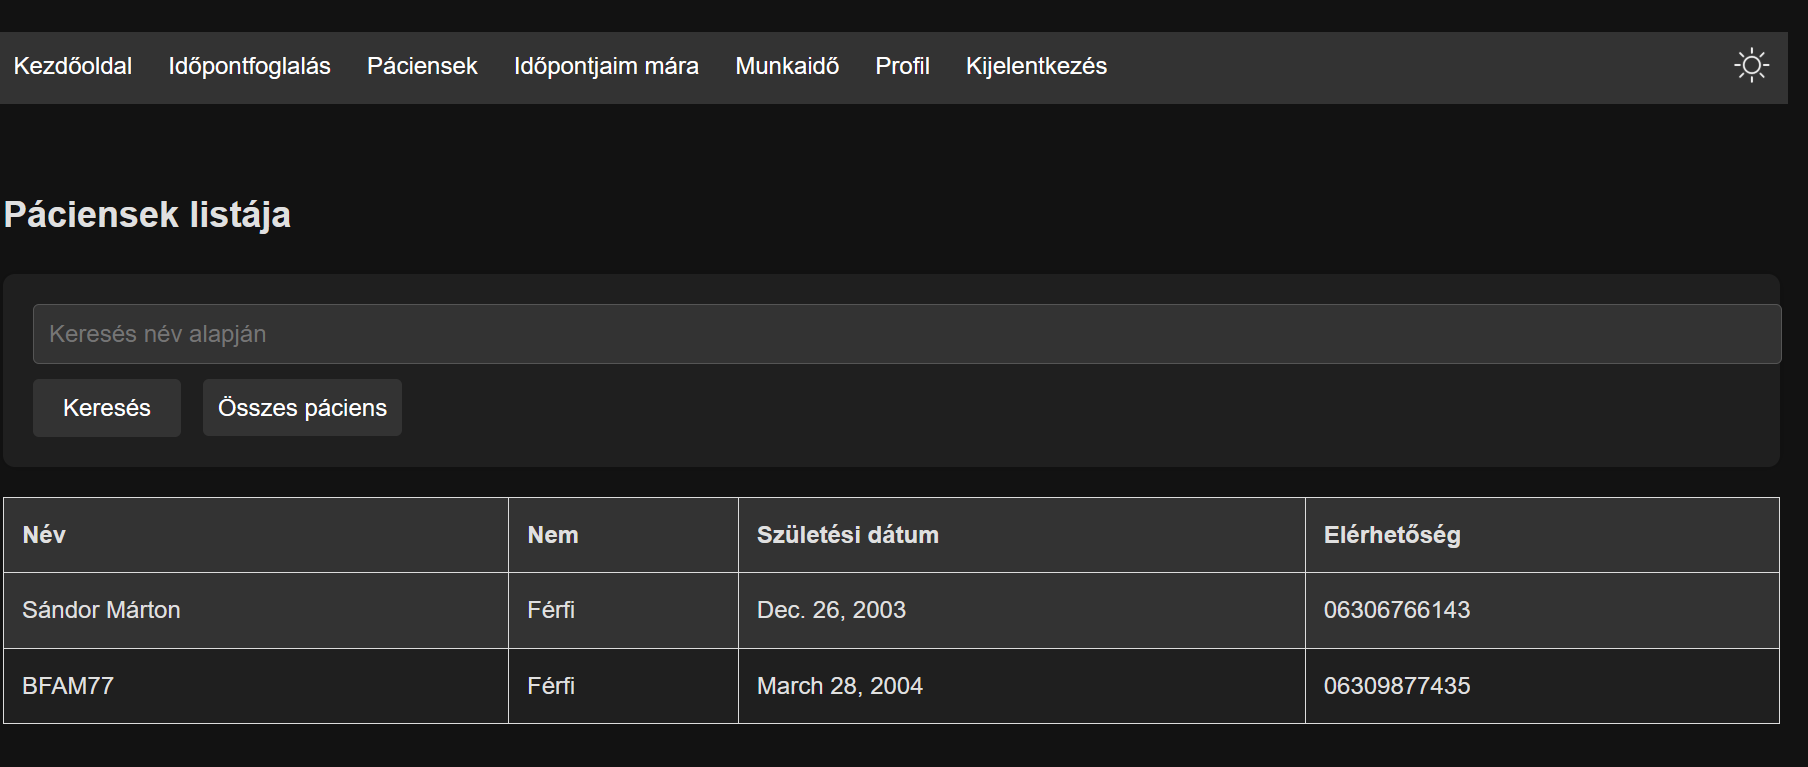
\includegraphics[width=1.0\textwidth]{patients_page.png}
\end{figure}

\section{Az "Időpontjaim mára" oldal}

Ezen az oldalon láthatja az orvos a hozzá foglalt időpontokat a megadott dátumon.

\begin{figure}[H]
	\caption{Az "Időpontjaim mára" oldal}
	\label{fig:idopontjaimmara}
	\centering
	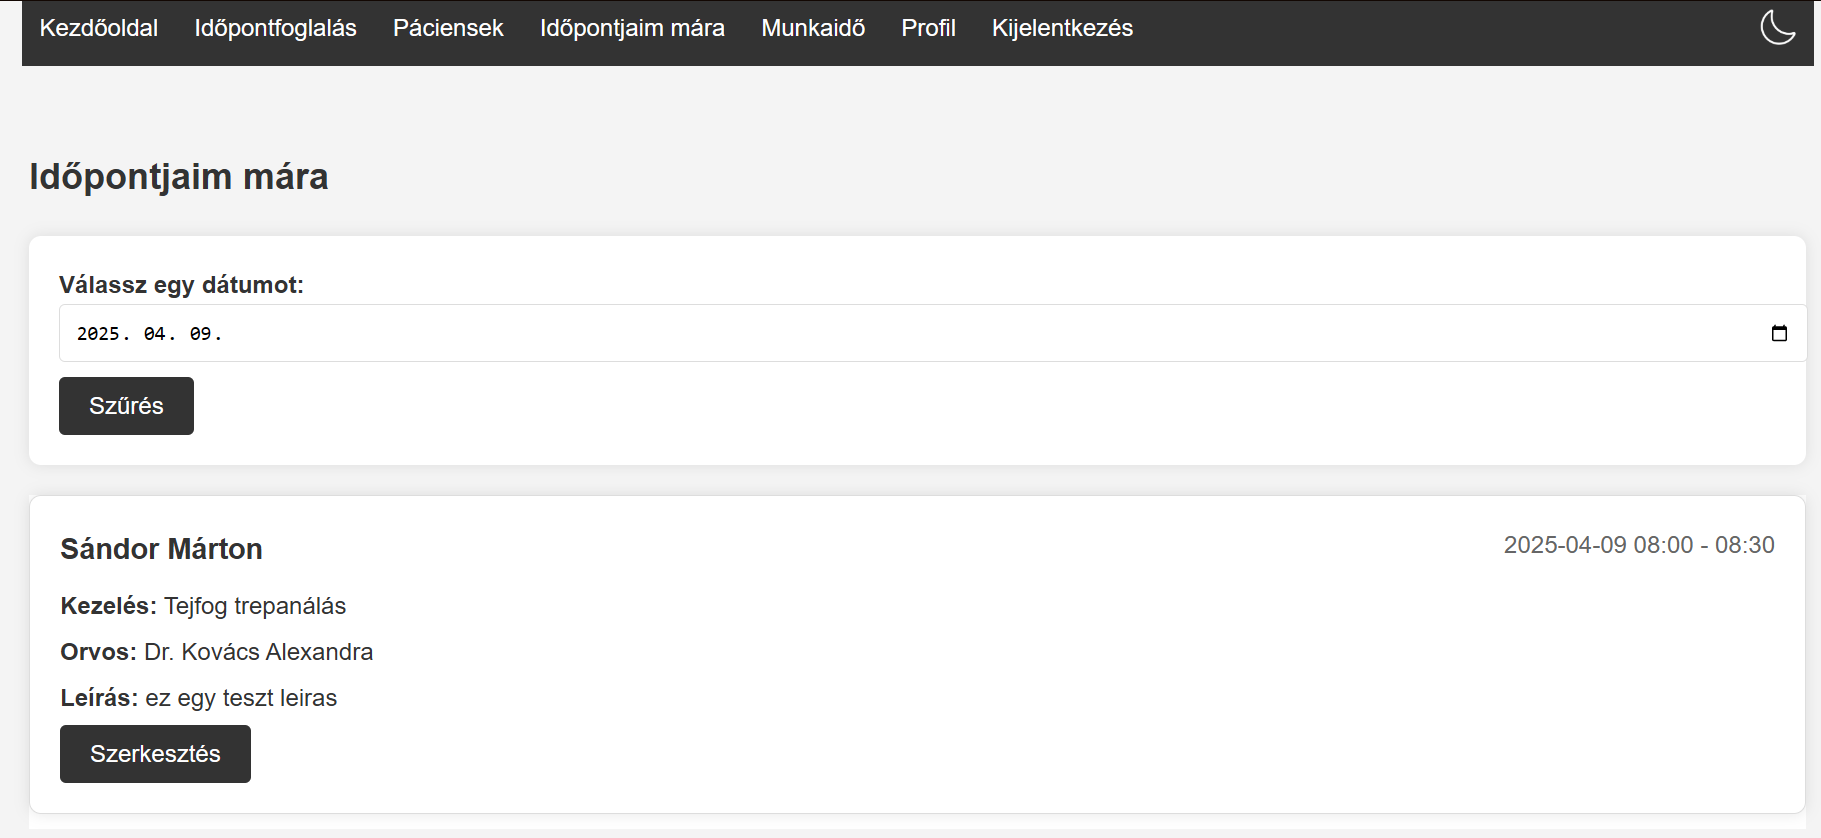
\includegraphics[width=1.0\textwidth]{idopontok_mara.png}
\end{figure}

A 6.2. ábrán látható módon jelennek meg az időpontok az oldalon. Alapértelmezetten a jelenlegi dátumra lefoglalt időpontok jelennek meg, viszont a beviteli mező segítségével a más dátumokra foglalt időpontokat is meg lehet nézni. Egy adott időpontnál a "Szerkesztés" gomb átnavigálja a felhasználót az "Időpont adatai" oldalra, ahol a "user" típusú felhasználók csak nézhetik az időpontjaik adatait, viszont az orvosoknak lehetőségük van szerkeszteni azok leírását. Így adható meg a páciens kezeléstörténete. Ez az oldal az "edit\_appointment.html" oldalon lett megvalósítva.

\begin{figure}[H]
	\caption{Az "Időpont adatai" oldal}
	\label{fig:idopontadatai}
	\centering
	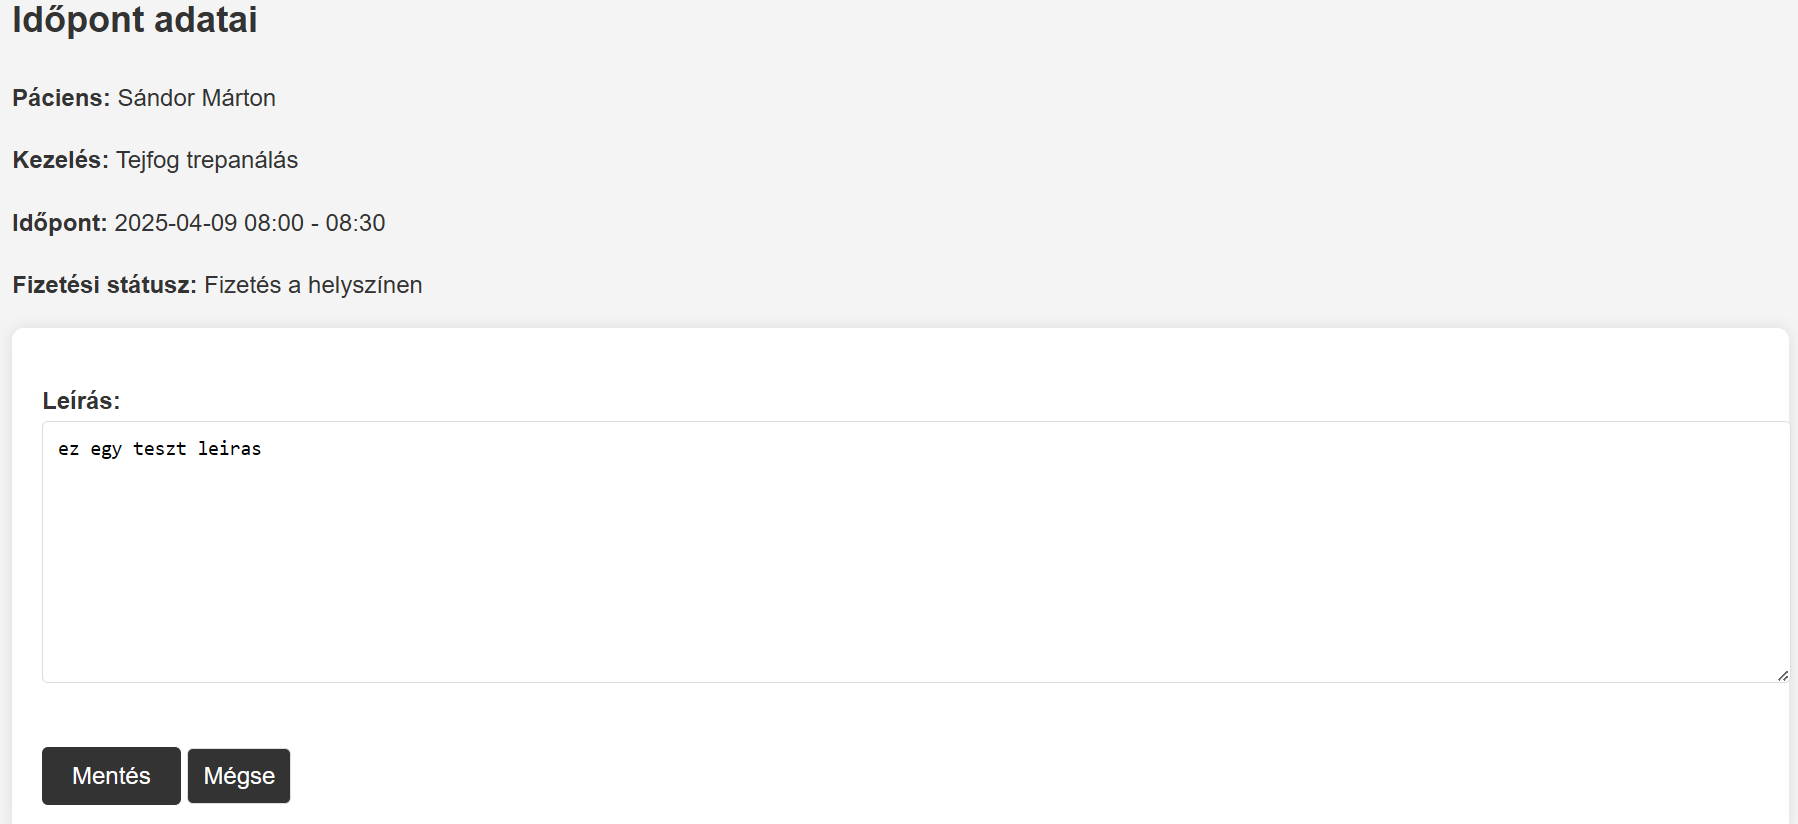
\includegraphics[width=1.0\textwidth]{idopont_szerkesztes.png}
\end{figure}

A "Metés" gombbal elmenthető a leírás amit az időponthoz rendeltünk, a "Mégse" gomb pedig visszanavigál az "Időpontjaim mára" oldalra.

\section{A "Munkaidő oldal"}

Az orvos a munkaidejét ezen az oldalon állíthatja be. Az oldal a "working\_hours.html" fájlban lett megvalósítva.

\begin{figure}[H]
	\caption{A munkaidő megadása}
	\label{fig:munkaidomegadasa}
	\centering
	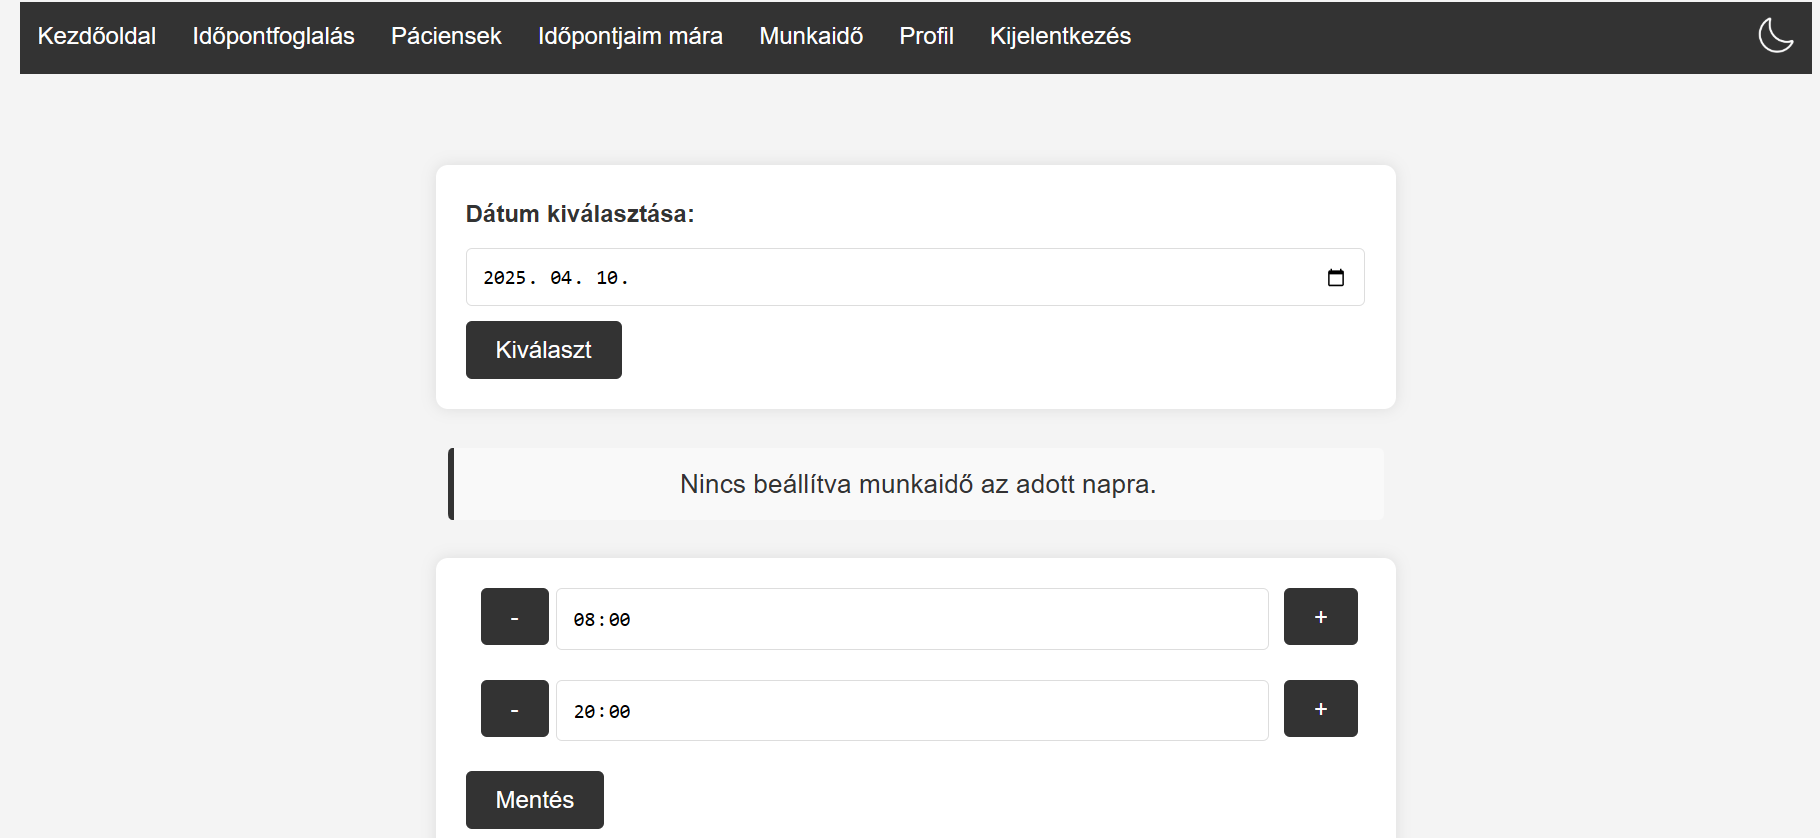
\includegraphics[width=1.0\textwidth]{working_hours.png}
\end{figure}

Amikor a felhasználó ellátogat az oldalra és kiválaszt egy dátumot, akkor a 6.4. ábrán látható kép fogadja. A rendelő 8:00-20:00 között van nyitva, tehát ennél korábbi kezdést, vagy későbbi végzést nem lehet beállítani munkaidőnek. A kezdés és végzés ideje a + és - gombokkal növelhető, vagy csökkenthető. Egy kattintás 15 perccel növeli, vagy csökkenti a beviteli mezőben látható időt. A beviteli mező ezeken a gombokon kívül mással nem szerkeszthető. Ez azért van, hogy a felhasználó ne adhasson meg magának olyan kezdési, vagy végzési időpontot, ami nem "kerek", és az időpontfoglalási rendszert összezavarná. A munkaidőt beállítani, vagy a már beállítottat szerkeszteni a "Mentés" gombbal lehet. Ennek a hatására az alkalmazás elmenti a "WorkingHours" model-be az orvos munkaidejét. Abban az esetben, ha még a kiválasztott napra nincs megadva az adott orvosnak munkaidő, akkor megjelenik a képen látható üzenet is az oldalon.

\section{Az orvosok Profil oldala}

Az orvosok profil oldala ugyan abban a fájlban lett megvalósítva ugyan azzal a működési elvvel, mint az az oldal, amit az 5.5. fejezetben bemutattam. Azonban ennél a típusú felhasználónál akadtak nehézségek, mivel a "DoctorForm" form töltődik be a "PatientForm" helyett, és ennek a formnak kezelnie kell képeket. Itt is a Django beépített fájlbeviteli mezőjét szerettem volna használni, de azt nem sikerült CSS kóddal designolnom, és nem nyújtott kellően szép látványt. A megoldásom az lett erre a problémára, hogy készítettem egy saját képbeviteli oldalt a "custom\_clearable\_file\_input.html" fájlba, készítettem a "forms.py"-ba egy osztályt hozzá, és a 6.5. ábrán látható módon beleraktam a "DoctorForm"-ba, hogy ezt használja a képek beviteléhez.

\begin{figure}[H]
	\caption{A "DoctorForm"}
	\label{fig:doctorform}
	\centering
	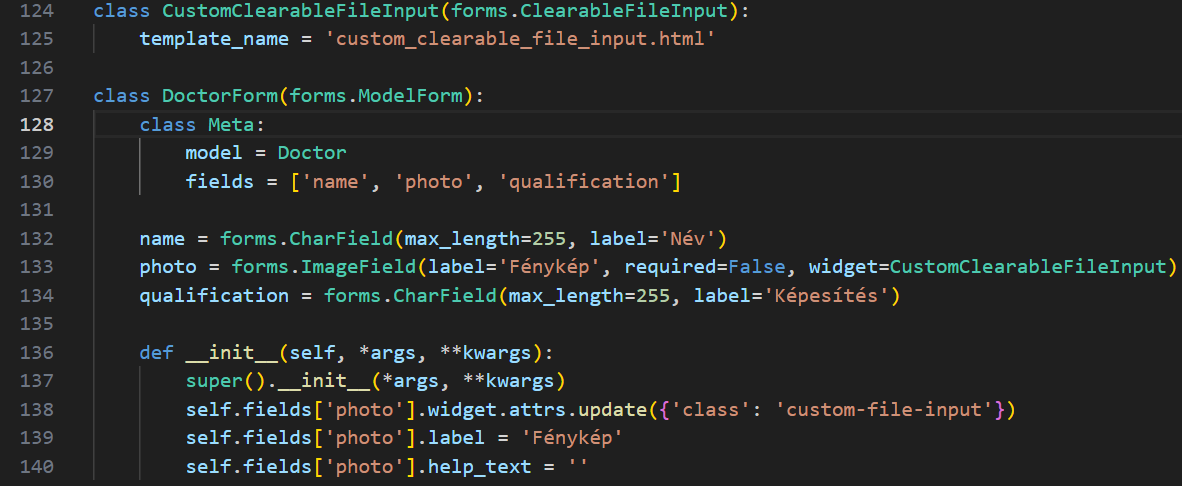
\includegraphics[width=1.0\textwidth]{doctor_form.png}
\end{figure}

Ezt már lehetett CSS kóddal designolni, így megoldódott a probléma, és a 6.6. ábrán látható is a munka eredménye.

\begin{figure}[H]
	\caption{A "DoctorForm" megjelenítése}
	\label{fig:doctorformview}
	\centering
	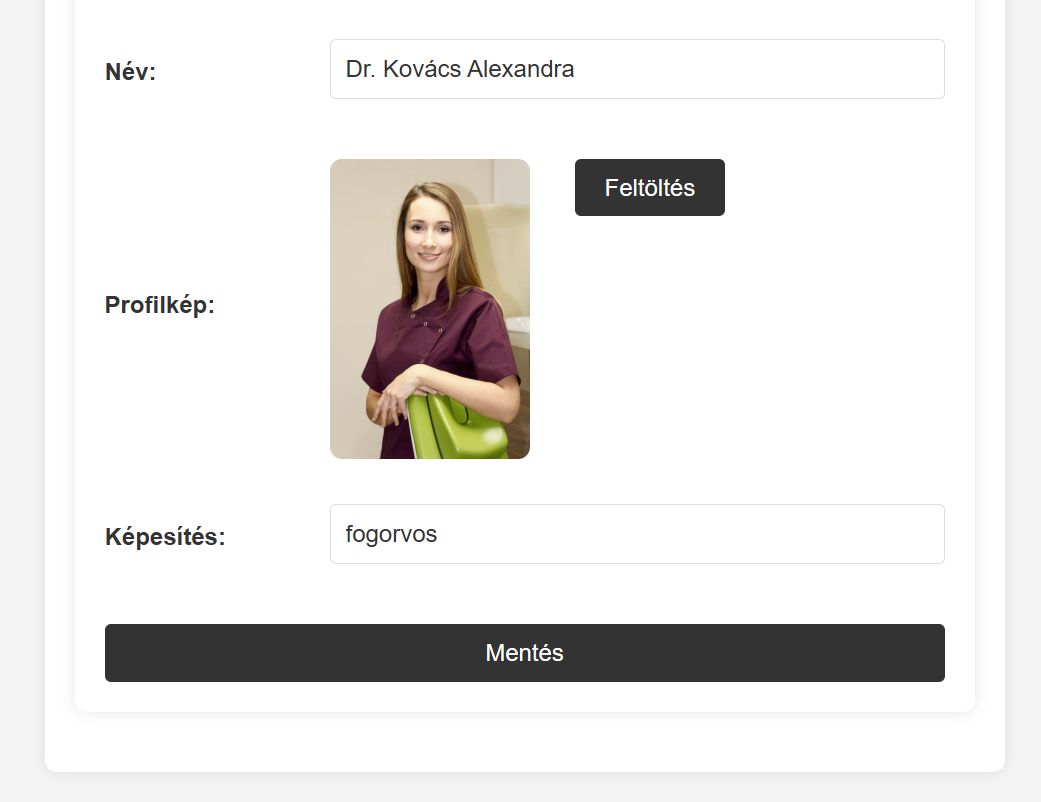
\includegraphics[width=1.0\textwidth]{doctor_form_view.png}
\end{figure}

A "Feltöltés" gomb megnyomásával ki lehet választani a képet, amit a felhasználó profilképként szeretne használni. Ez a kép jelenik meg a pácienseknek az időpont foglalásnál is, amikor az orvos kiválasztására kerül sor. A program a profilképeket a rendelo/media/doctor\_pictures mappába menti.



